\documentclass[10pt]{beamer}

% mac版,texShop 中Typeset选择 XeLaTex 

%%%%%%%%%%%%%%%%%%%%%%%%%%%%%%%%%%%%%
\usepackage[slantfont,boldfont]{xeCJK}
%\input{xecjkfonts},CJKtextspaces
\setCJKmainfont{STKaiti}   % STFangsong 设置缺省中文字体
\setCJKmonofont{SimSun}   % 设置等宽字体
\setmainfont{Times} % 英文衬线字体
\setmonofont{Times} % 英文等宽字体
\setsansfont{Times} % 英文无衬线字体
%%%%%%%%%%%%%%%%%%%%%%%%%%%%%%%%%%%%%%

\mode<presentation> {
  %\usetheme{Madrid}
  %\usetheme{Singapore}
  \usetheme{Warsaw}
  \setbeamercovered{transparent}
 % \usefonttheme[onlymath]{serif}  
 \usefonttheme{professionalfonts}%{structurebold}
 % \usefonttheme[onlymath]{structurebold}
  \usecolortheme{rose}
}

\usepackage[english]{babel}
%\usepackage[latin1]{inputenc}

%\usepackage{times}
%\usepackage[T1]{fontenc}


%\usepackage{epsfig}
\usepackage{graphics}
\usepackage{color}
\usepackage{amsmath,amssymb,mathrsfs}
\usepackage{amsfonts,stmaryrd}
%\usepackage{thmmarks}
%\usepackage{}



\newcommand\frakfamily{\usefont{U}{yfrak}{m}{n}}
\DeclareTextFontCommand{\textfrak}{\frakfamily}
\def\diag{\mathrm{diag}}


\title[数值计算方法]{数值计算方法}
\subtitle{-直接法求解线性方程组}


\subject{Talks}

% If you have a file called "university-logo-filename.xxx", where xxx
% is a graphic format that can be processed by latex or pdflatex,
% resp., then you can add a logo as follows:

% \pgfdeclareimage[height=0.5cm]{university-logo}{university-logo-filename}
% \logo{\pgfuseimage{university-logo}}

%\pgfdeclareimage[height=0.5cm]{university-logo}{ncsu_logo}
%\logo{\pgfuseimage{university-logo}}

% Delete this, if you do not want the table of contents to pop up at
% the beginning of each subsection:
%\AtBeginSubsection[] {
%  \begin{frame}<beamer>
%    \frametitle{Outline}
%    \tableofcontents[currentsection,currentsubsection]
%  \end{frame}
%}

% If you wish to uncover everything in a step-wise fashion, uncomment
% the following command:

% \beamerdefaultoverlayspecification{<+->}


\setbeamertemplate{theorems}[numbered]
\setbeamertemplate{caption}[numbered]


\newtheorem{proposition}[theorem]{Proposition}

%%%%%%%%%%%%%%%%%%%%%%%%%%%
% REMARK-STYLE-ENVIRONMENTS %
%%%%%%%%%%%%%%%%%%%%%%%%%%%
\newcounter{remark}
% \numberwithin{theorem}{section}
\def\openrem#1#2{\refstepcounter{remark}\bigskip

{\noindent\bf#1~\theremark\if#2!{. }\else{ (#2).}\fi}
\it}
\def\thmskip{}
\newenvironment{remark}[1][!]{\openrem{Remark}{#1}}{\thmskip}

%%%%%%%%%%%%%%%%%%%%%%%%%%%%
%% AlGORITHM-STYLE-ENVIRONMENTS %
%%%%%%%%%%%%%%%%%%%%%%%%%%%%
\newcounter{algorithm}
% \numberwithin{theorem}{section}
\def\openalg#1#2{\refstepcounter{algorithm}\bigskip

{\noindent\bf#1~\thealgorithm\if#2!{. }\else{ (#2).}\fi}
\it}
\def\thmskip{}
\newenvironment{algorithm}[1][!]{\openrem{Algorithm}{#1}}{\thmskip}
%
%
%%%%%%%%%%%%%%%%%%%%%%%%%%%%
%% Result-STYLE-ENVIRONMENTS %
%%%%%%%%%%%%%%%%%%%%%%%%%%%%
%\newcounter{result}
%\def\openrem#1#2{\refstepcounter{result}\bigskip
%{\noindent \it \bfseries#1~\theremark\if#2!{. }\else{ (#2). }\fi}}
%\newenvironment{result}[1][!]{\openrem{Result}{#1}}{\qed}




%%%%%%%%%%%%%%%%%%%%%%%%%%%
%Redefine the Symbols%
%%%%%%%%%%%%%%%%%%%%%%%%%%%

\def\mathbi#1{\textbf{\em #1}}

% integrals
\def\dx{\,{\rm d}x}
\def\dxb{\,{\rm d}\boldsymbol{x}}
\def\dy{\,{\rm d}y}
\def\dt{\,{\rm d}t}
\def\ds{\,{\rm d}s}
\def\du{\,{\rm d}u}

\def\dr{\,{\rm d}r}
\def\dtheta{\,{\rm d}\theta}

\def\dd{{\rm d}}

\def\intOm{\int_{\Omega}}
\def\intbOm{\int_{\partial \Omega}}

% differences
\def\Dx{\Delta x}
\def\Dt{\Delta t}
\def\D{\Delta}


% operators
\def\Ls{\mathscr{L}}

% matirices
\def\Js{\mathscr{J}}


%fields%
\def\R{\mathbb{R}}
\def\N{\mathbb{N}}
\def\Z{\mathbb{Z}}

%Spaces%
\def\H{\mathbb{H}}
\def\L{\mathbb{L}}
\def\P{\mathbb{P}}


\def\U{\mathbb{U}}
\def\V{\mathbb{V}}
\def\W{\mathbb{W}}
\def\X{\mathbb{X}}
\def\Y{\mathbb{Y}}

\def\Cinfty{C^\infty}




%vectors%
\def\ab{\boldsymbol{a}}
\def\bb{\boldsymbol{b}}
\def\cb{\boldsymbol{c}}
\def\db{\boldsymbol{d}}
\def\eb{\boldsymbol{e}}
\def\fb{\boldsymbol{f}}
\def\gb{\boldsymbol{g}}
\def\hb{\boldsymbol{h}}
\def\nb{\boldsymbol{n}}
\def\rb{\boldsymbol{r}}
\def\sb{\boldsymbol{s}}


\def\ub{\boldsymbol{u}}
\def\vb{\boldsymbol{v}}
\def\wb{\boldsymbol{w}}
\def\xb{\boldsymbol{x}}
\def\yb{\boldsymbol{y}}
\def\zb{\boldsymbol{z}}

\def\Bb{\boldsymbol{B}}
\def\Cb{\boldsymbol{C}}
\def\Eb{\boldsymbol{E}}
\def\Fb{\boldsymbol{F}}
\def\Ib{\boldsymbol{I}}
\def\Kb{\boldsymbol{K}}
\def\Ob{\boldsymbol{O}}
\def\Qb{\boldsymbol{Q}}
\def\Rb{\boldsymbol{R}}
\def\Sb{\boldsymbol{S}}
\def\Ub{\boldsymbol{U}}
\def\Vb{\boldsymbol{V}}
\def\Wb{\boldsymbol{W}}
\def\Xb{\boldsymbol{X}}
\def\Yb{\boldsymbol{Y}}
\def\Zb{\boldsymbol{Z}}

%domains%
\def\Om{\Omega}
\def\bd{\partial}
\def\bOm{\bar{\Omega}}

%bold symbols%
\def\alphab{\boldsymbol{\alpha}}
\def\phib{\boldsymbol{\varphi}}

%energy%
\def\Jc{\mathcal{J}}
\def\Oc{\mathcal{O}}

%Greeks%
\def\vphi{\varphi}

%Special Functions%
\def\supp{\rm{supp}}
\def\sym{\rm{sym}}

\def\gradu{\nabla u}
\def\gradv{\nabla v}

%Mesh%
\def\Ts{\mathcal{T}}

\def\mach{\rm{mach}}


\begin{document}

\setbeamertemplate{itemize item}[triangle]

\begin{frame}
\titlepage
\end{frame}


\begin{frame}
  \frametitle{本节概要}
  \tableofcontents%[pausesections]
  % You might wish to add the option [pausesections]
%  \begin{itemize}
%  \item 显示Euler法及其误差分析
%  \item Taylor展开法
%  \item 
%  \end{itemize}
\end{frame}

\section{求线性方程组概述}

\begin{frame}
\frametitle{求解线性方程组概述}
许多物理问题,包括力学和电磁学的问题,都可以由微分方程进行数学建模,而求解这些微分方程往往利用的是数值方法,主要是离散化的方法。利用离散化的方法解微分方程就会导出大规模的线性方程组,因此我们需要对求解大型的线性方程组的问题进行研究。\\
\vspace{0.2cm}
求解线性方程组有很多方法,但不同方法的计算效率差别很大,有一些形式非常漂亮的数学上的结论在实际求解线性方程组的时候是不适用的,比如著名的Cramer(克拉默)法则:


\end{frame}


\begin{frame}
\frametitle{一个无效的算法}
\begin{theorem}[Cramer法则]
假设有一个由$n$个方程和$n$个未知数构成的线性方程组$Ax = b$,并且$A$是满秩的,即$D = \det (A) \neq 0$,则这个方程组的解满足
\begin{equation}
x_i = \frac{D_i}{D}, i = 1,2, \ldots, n,
\end{equation}
其中$D_i = \det (A_i)$,$A_i$是$A$的第$i$列用$b$代替所得的矩阵。
\end{theorem}

这个漂亮的定理在实际当中是无法使用的,问题就在于计算量。对于$n$阶行列式,大致需要$n!$次的乘除法运算,这个数字是非常大的。

比如假设$n = 100$,用目前世界上排名前十的巨型计算机进行计算,速度稳定在$10^{33}$次/秒,则算一次$100$阶行列式的时间是$3\times10^{119}$年,而地球的年龄是$4.5\times 10^9$年。

这就是为什么我们经常说数学上等价计算上不等价,也是为什么我们需要好的算法来处理那怕是非常简单的问题。
\end{frame}



%%%%%%%%%%%%%%%%%%%%%%%%%%%%%%%%%%%%%%%%%%


\section{高斯消元}

\begin{frame}
\frametitle{高斯消元的理论基础}
解线性方程组最基本的方法是高斯消元法,高斯消元法是基于以下线性方程组的等价性的,也就是说我们对于一个方程组作以下变换所得到的新的方程组与原方程组等价:
\begin{itemize}
\item 将两个方程交换位置
\item 将一个方程两边同时乘以一个非零的数
\item 将一个方程两边同时乘以一个数加到另一个方程两边
\end{itemize}

根据以上方程组的等价性,我们可以构造高斯消元法,首先举一个简单的例子。
\end{frame}


\begin{frame}
\frametitle{一个简单的例子}
\begin{example}
解方程组
\begin{align}
x + y &= 3, \nonumber \\
3x - 4y &= 2.
\end{align}
\end{example}
将第一个方程乘以$-3$加到第二个方程上,我们得到等价的方程组
\begin{align}
x + y &= 3, \nonumber \\
- 7y &= -7.
\end{align}
从最后一个方程开始求解,首先得到
\begin{figure}
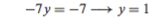
\includegraphics[width=3.5cm]{figs/2_1_Gaussian_Elimi_Eq_1} 
%\caption{$f(x) = x^3 + x -1$的图像} 
\end{figure}
将结果回带到第一个方程后得到
\begin{figure}
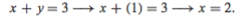
\includegraphics[width=5.5cm]{figs/2_1_Gaussian_Elimi_Eq_2} 
%\caption{$f(x) = x^3 + x -1$的图像} 
\end{figure}
\end{frame}


\begin{frame}
\frametitle{高斯消元的增广矩阵形式}
利用系数矩阵和右端项组成的增广矩阵来进行高斯消元,表示会更为简便。例如上面的例子,我们得到
\begin{figure}
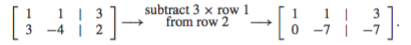
\includegraphics[width=8cm]{figs/2_1_Gaussian_Elimi_Eq_3} 
\end{figure}
由于增广矩阵中不含有未知数,所以在手动高斯消元和高斯消元的分析中有更多的运用。

在上面的例子中,我们实际上做了两件事情,
\begin{enumerate}
\item 将系数矩阵的主对角元下面的元素消为$0$,从而得到阶梯状的系数矩阵;
\item 通过回带,先求出后面的未知数的值,再代入上面一个方程求出前面的未知数的值。
\end{enumerate}
这两个步骤就构成基本的高斯消元法。
\end{frame}


\begin{frame}
\frametitle{高斯消元法的一般形式}
现在考虑由$n$个方程并含有$n$个未知数的的线性方程组$Ax = b$,利用增广矩阵,这样的方程组一般写为
\begin{figure}
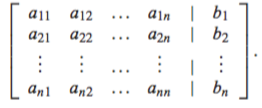
\includegraphics[width=4.5cm]{figs/2_1_2_Gaussian_Elimi_Augmented} 
\end{figure}

对于消去的步骤,我们可以简单的描述为
\begin{algorithm}\\
\rm{for} $j = 1 : n-1$ \\
\quad 消去系数矩阵中第$j$列中排在$a_{jj}$下面的各元素。 \\
\rm{end} \\
\end{algorithm}
\end{frame}


\begin{frame}
\frametitle{高斯消元法的一般形式}
上面的算法可以更详细的描述为
\begin{algorithm}\\
\rm{for} $j = 1 : n-1$ \\
\quad \rm{for} $i  = j+1 : n$ \\
\quad \quad 消去系数矩阵中的$a_{ij}$。 \\
\quad \rm{end} \\
\rm{end} \\
\end{algorithm}

我们将第$i$行乘以相应的系数加到第$i+1,\ldots, n$行上的办法来完成算法中消去系数矩阵中的$a_{ij}$的工作。
\end{frame}

\begin{frame}
\frametitle{高斯消元法}
例如消去第一列上$a_{11}$以下的元素,我们首先将第一行乘以$-\frac{a_{21}}{a_{11}}$加到第二行,得到
\begin{figure}
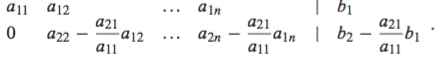
\includegraphics[width=7cm]{figs/2_1_2_Gaussian_Elimi_Augmented-2} 
\end{figure}
我们对第$3, \ldots, n$行重复这个步骤,例如对于第$i$行,我们有
\begin{figure}
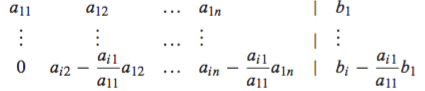
\includegraphics[width=7cm]{figs/2_1_2_Gaussian_Elimi_Augmented-3} 
\end{figure}
只要$a_{11}$不为$0$,这个步骤就可以进行下去。
\end{frame}


\begin{frame}
\frametitle{高斯消元法的运算量}
通过上面的步骤,我们可以得到这样形式的增广矩阵
\begin{figure}
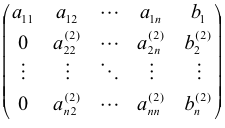
\includegraphics[width=5cm]{figs/2_1_2_Gaussian_Elimi_Augmented-4} 
\end{figure}
在这个消去过程中的每一步,我们用了$1$次除法(例如计算$\frac{a_{21}}{a_{11}}$),$n$次乘法(例如计算$-\frac{a_{21}}{a_{11}} a_{1j}$,$i = 2, \ldots, n$,以及$-\frac{a_{21}}{a_{11}} b_1$),以及$n$次加法(例如计算$a_{2j} - \frac{a_{21}}{a_{11}} a_{1i}$,$j = 2, \ldots, n$,以及$b_2-\frac{a_{21}}{a_{11}} b_1$)。也就是说总共做了$2n+1$次运算。而这个消去过程有$n-1$步(因为消去了$n-1$行的中第一列的元素),所以这个过程总过做了$(2n+1) \times (n-1)$次运算。
\end{frame}


\begin{frame}
\frametitle{高斯消元法的运算量}
接下来我们可以将第$2$行乘以相应的系数加到后面的行上来消去第$2$列上$a_{22}$以下的元素。假设消去过程进行到了第$j$行,则利用第$j$行消去第$i$行($i > j$)的过程可以用以下形式表示
\begin{figure}
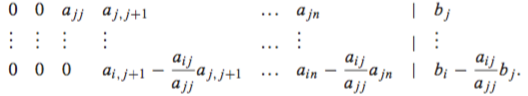
\includegraphics[width=9cm]{figs/2_1_2_Gaussian_Elimi_Augmented-5} 
\end{figure}
这里的每一步中,我们需要做$1$次除法,$n-j+1$次乘法和$n-j+1$次加法,所以消去第$j$列$a_{jj}$下面的所有元素需要$(2\times (n-j+1)+1) \times (n-j)$ 次的运算。

\begin{remark}
我们注意到,高斯消元能够进行下去的条件是第$j$步时,$a_{jj} \neq 0$,这里$a_{jj}$是经过消去之后所得到的系数矩阵对角线上元,这样的元称为主元。并不是所有的线性方程组在消去过程中主元都能够保持不为$0$的,对于主元出现$0$的情况,我们将在后面讨论,这里我们假设所有的主元都不为$0$。
\end{remark}
\end{frame}


\begin{frame}
\frametitle{基本高斯消元法具体算法}
有了上面的推导,我们可以得到基本高斯消元法的算法。
\begin{algorithm}[基本高斯消元]\\
\rm{for} $j = 1 : n-1$\\
\quad \rm{if} $|a_{jj}| < \epsilon$\\
\quad \quad 主元接近于$0$,结束程序\\
\quad \rm{if} $i = j+1 : n$ \\
\quad \quad ${\rm{mult}} = \frac{a_{ij}}{a_{jj}}$\\
\quad \quad \rm{for} $k = j+1 : n$\\
\quad \quad \quad $a_{i,k} = a_{i,k} - \rm{mult} \times a_{jk}$ \\
\quad \quad \rm{end}\\
\quad \quad $b_i = b_i - \rm{mult} \times b_j$\\
\quad \rm{end}\\
\rm{end}\\
\end{algorithm}
\end{frame}


\begin{frame}
\frametitle{基本高斯消元法具体算法}
上面的算法我们注意到两个问题:
\begin{itemize}
\item 第一是我们实际上并没有将对角线以下的元素设为$0$,这是因为在最后的回代过程中,我们实际上不会用到对角线以下的元素的值,因此为了提高效率,我们没有做这样一个赋值运算;
\item 第二,对于主元接近于$0$的情况,我们直接结束了程序,这是因为我们后面会看到主元过小会导致严重的计算误差。
\end{itemize}
\end{frame}


\begin{frame}
\frametitle{消元步骤的运算量}
上面我们考虑了高斯消元每一步的运算量,我们用下面的形式把每一步的运算量非常直观的表示出来
\begin{figure}
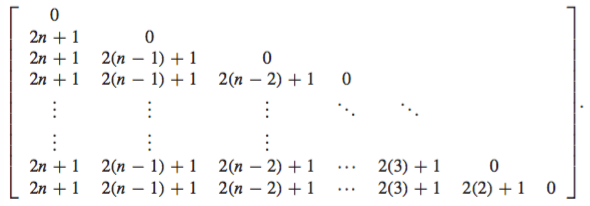
\includegraphics[width=9cm]{figs/2_1_2_Gaussian_Elimi_Operation_Counts} 
\end{figure}
\end{frame}


\begin{frame}
\frametitle{消元步骤的运算量}
对于总的运算量,我们可以进行如下计算
\begin{figure}
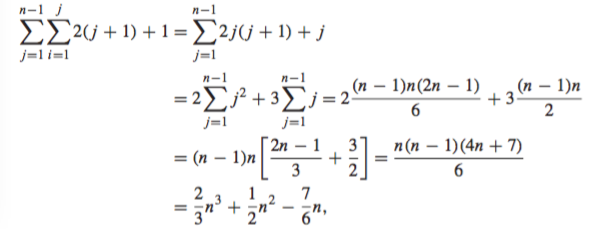
\includegraphics[width=9cm]{figs/2_1_2_Gaussian_Elimi_Operation_Counts-2} 
\end{figure}
这里我们用到了
\begin{align}
\sum_{i = 1}^n i     &= \frac{n(n+1)}{2}, \\
\sum_{i = 1}^n i^2 &= \frac{n(n+1)(2n+1)}{6}. 
\end{align}
\end{frame}


\begin{frame}
\frametitle{回代步骤的运算量}
除了消元,我们还需要回代的过程,这时我们需要解方程组
\begin{figure}
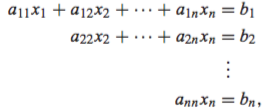
\includegraphics[width=4.5cm]{figs/2_1_2_Gaussian_Elimi_Operation_Counts-3} 
\end{figure}
也就是计算
\begin{figure}
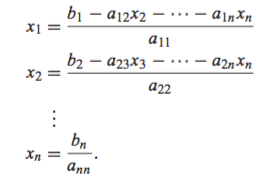
\includegraphics[width=4.5cm]{figs/2_1_2_Gaussian_Elimi_Operation_Counts-4} 
\end{figure}
\end{frame}


\begin{frame}
\frametitle{回代步骤的运算量}
因此,回代步骤的运算量为
\begin{equation}
1 + 3 + 5 + \ldots + (2n-1) = 2\sum_{i = 1}^n i - 1 = n^2.
\end{equation}

而回代步的算法为
\begin{algorithm}[回代算法]\\
\rm{for} $i = n : -1 : 1$\\
\quad \rm{for} $j = i+1 : n$ \\
\quad \quad $b_i = b_i - a_{ij} \times x_j $\\
\quad \rm{end}\\
\quad $x_i = \frac{b_i}{a_{ii}}$ \\
\rm{end}\\
\end{algorithm}
\end{frame}


\begin{frame}
\frametitle{高斯消元法总的运算量}
高斯消元法总的运算量由消去步骤和回代步骤运算量的和决定,但是我们发现,高斯消元法运算量中占主导的实际上是消去步骤中的$\frac{2}{3} n^3$,随着$n$变大,其它项与这个主项的差就越大。如果我们忽略常数$\frac{2}{3}$,我们可以说高斯消元法总的运算量与$n^3$是同阶无穷大,即总的运算量是$O(n^3)$。

运算量的阶数往往又称为计算复杂度(或者更准确的说是计算复杂度的一种度量),因此,高斯消元法是一种具有$O(n^3)$计算复杂度的算法,相比于克拉默法则的$O(n!)$的复杂度,高斯消元是一种非常有效的算法。
\end{frame}




%%%%%%%%%%%%%%%%%%%%%%%%%%%%%%%%%%%%%%%%%%

\section{$LU$分解}

\begin{frame}
\frametitle{$LU$分解的动机}
通过对高斯消元法的讨论,我们发现,高斯消元法主要的计算复杂度在于消去的步骤,而回代的步骤相对来说计算复杂度比较低。考虑这样一个问题,如果我们需要解许多系数矩阵一样而右端项不一样的线性方程组
\begin{align}
Ax &= b_1 \nonumber \\
 Ax &= b_2 \nonumber \\
&\vdots \nonumber \\
Ax & = b_k
\end{align}
如果每一次都进行一次完整的高斯消元,那么计算量可以达到$k n^3$。
\end{frame}


\begin{frame}
\frametitle{$LU$分解的动机}
我们考虑回代过程,回代过程的计算量比较低的原因是我们通过消去过程将系数矩阵化为了一个上三角矩阵(即对角线以下的元素均为$0$的矩阵)。如果我们可以将原来的系数矩阵$A$化为两个矩阵$L$和$U$的乘积,其中$L$是一个下三角矩阵(即对角线以上的元素均为$0$的矩阵),其中$U$是一个上三角矩阵(即对角线以上的元素均为$0$的矩阵),那么给定一个右端项$b$,我们都可以将解线性方程组的过程变为两个回代的过程,即解以下两个方程组
\begin{align}
Ly & = b \\
Ux & = y,
\end{align}
进而得到原方程组的解,这样就大大提高了解方程组的效率。下面我们就通过例子来探讨如何将一个方程组的系数矩阵$A$化为特定形式的$L$与$U$的乘积。

\end{frame}


\begin{frame}
\frametitle{$LU$分解的数学基础}
$LU$分解能够实现的根本原因是我们在消去步骤时对矩阵进行的初等变换是可以用矩阵左乘一个特殊的下三角矩阵实现的。如果我们令$L_{ij}(-c)$表示对角线上元素均为$1$,而其它位置元素除第$(i,j)$位置上的元素为$-c$之外均为$0$的矩阵。那么将$A$矩阵第$j$行乘以$-c$倍加到第$i$行可以表示为$L_{ij}(-c)A$。例如$A$是$3\times3$的矩阵,左乘$L_{21}(-c)$,我们得到
\begin{figure}
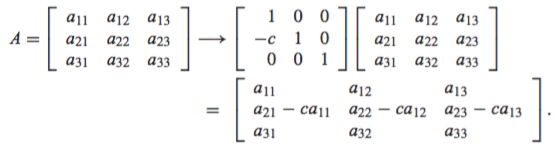
\includegraphics[width=9cm]{figs/2_2_LU-1} 
\end{figure}
\end{frame}


\begin{frame}
\frametitle{利用矩阵乘法表示高斯消元}
考虑矩阵
\begin{figure}
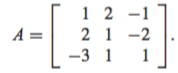
\includegraphics[width=3cm]{figs/2_2_LU-2} 
\end{figure}
将第$1$行乘以$-2$加到第$2$行上,即$L_{21}(-2) A$得到
\begin{figure}
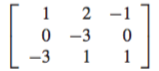
\includegraphics[width=3cm]{figs/2_2_LU-3} 
\end{figure}
\end{frame}

\begin{frame}
\frametitle{利用矩阵乘法表示高斯消元}
再将矩阵第$1$行乘以$3$加到第$3$行上,即$L_{31}(3)L_{21}(-2) A$得到
\begin{figure}
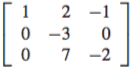
\includegraphics[width=3cm]{figs/2_2_LU-4} 
\end{figure}
将上面这个矩阵的第$2$行乘以$\frac{7}{3}$加到第$3$行,即$L_{32}(\frac{7}{3})L_{31}(3)L_{21}(-2) A$得到
\begin{figure}
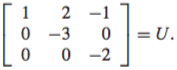
\includegraphics[width=4cm]{figs/2_2_LU-5} 
\end{figure}
即$L_{32}(\frac{7}{3})L_{31}(3)L_{21}(-2) A = U$。
\end{frame}


\begin{frame}
\frametitle{$L_{ij}(-c)$的逆}
在数学上,$L_{ij}(-c)$是初等矩阵的一种,而这种初等矩阵的逆非常特殊,我们有
\begin{equation}
\big[L_{ij}(-c) \big]^{-1} = L_{ij}(c) .
\end{equation}
例如我们可以验证
\begin{figure}
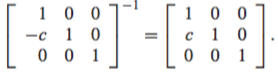
\includegraphics[width=5cm]{figs/2_2_LU-6} 
\end{figure}
\end{frame}


\begin{frame}
\frametitle{$L_{ij}(-c)$的乘积}
由此,对于上面的例子,我们有
\begin{align}
L_{32}(\frac{7}{3})L_{31}(3)L_{21}(-2) A &= U \nonumber \\
A &= L_{21}(2)L_{31}(-3)L_{32}(-\frac{7}{3})U.
\end{align}
对于$L_{ij}(c)$这样的矩阵的乘积又有特殊的性质,例如
\begin{figure}
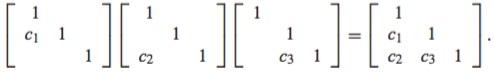
\includegraphics[width=8cm]{figs/2_2_LU-7} 
\end{figure}
\end{frame}


\begin{frame}
\frametitle{矩阵的$LU$分解}
这样我们就得到了矩阵的$LU$分解,以上面的矩阵$A$为例,我们有
\begin{figure}
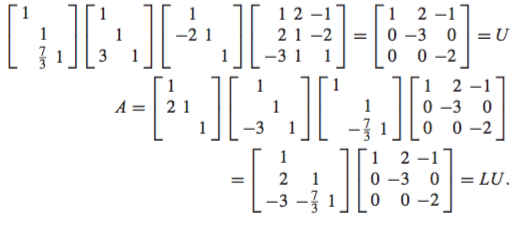
\includegraphics[width=9cm]{figs/2_2_LU-8} 
\end{figure}
也就是说,如果我们在高斯消元的同时可以保存每一步消元时所乘的系数,我们就可以很简单的得到系数矩阵的$LU$分解。
\end{frame}

%%%%%%%%%%%%%%%%%%%%%%%%%%%%%%%%%%%%%%%%%%

\section{吞噬现象}

\begin{frame}
\frametitle{主元近似为零}
回忆高斯消元法的算法,当主元非常小的时候我们会跳出循环并输出算法失败的信息,这样做的原因就是当主元非常小的时候会产生很大的计算误差。这里我们用一个简单的例子展现这个问题。
\begin{example}
解以下方程组
\begin{align}
10^{-20}x_1 + x_2 &= 1, \nonumber \\
x_1 + 2x_2 & = 4.
\end{align}
\end{example}

我们用三种不同的方法来解这个方程组:
\begin{itemize}
\item 手动解方程组;
\item 用IEEE双精度计算机解方程组;
\item 将第二个方程换为第一个方程后,用IEEE双精度计算机解方程组。
\end{itemize}
\end{frame}


\begin{frame}
\frametitle{手动解方程组}
我们将方程组写为增广矩阵形式,得到
\begin{figure}
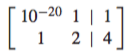
\includegraphics[width=2cm]{figs/2_3_Swamping-1} 
\end{figure}
将第一行乘以$-10^{20}$加到第二行上得到
\begin{figure}
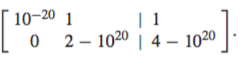
\includegraphics[width=3.5cm]{figs/2_3_Swamping-2} 
\end{figure}
回代得到
\begin{figure}
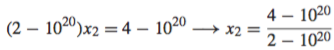
\includegraphics[width=5cm]{figs/2_3_Swamping-3} 
\end{figure}
\end{frame}


\begin{frame}
\frametitle{手动解方程组}
将$x_2$的值代回到变换后的第一个方程得到
\begin{figure}
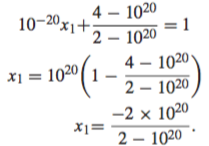
\includegraphics[width=4cm]{figs/2_3_Swamping-4} 
\end{figure}
从而精确解为
\begin{figure}
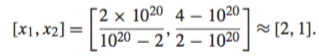
\includegraphics[width=5cm]{figs/2_3_Swamping-5} 
\end{figure}
\end{frame}


\begin{frame}
\frametitle{用IEEE双精度计算机解方程组}
与手动解方程组一样,我们将方程组写为增广矩阵形式,得到
\begin{figure}
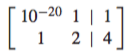
\includegraphics[width=2cm]{figs/2_3_Swamping-1} 
\end{figure}
将第一行乘以$-10^{20}$加到第二行上得到
\begin{figure}
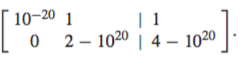
\includegraphics[width=3.5cm]{figs/2_3_Swamping-2} 
\end{figure}
但是由于在IEEE双精度表示中$2-10^{20}$与$-10^{20}$相等,而$4-10^{20}$与$-10^{20}$相等(相当于小数被大数吃掉),因此第二个方程等价于
\begin{equation}
-10^{20} x_2 = -10^{20}  \rightarrow x_2 = 1.
\end{equation}
\end{frame}


\begin{frame}
\frametitle{用IEEE双精度计算机解方程组}
将$x_2$代入到变换后的第一个方程中,我们有
\begin{equation}
10^{-20} x_1 +1 = 1  \rightarrow x_1 = 0.
\end{equation}
因此解为
\begin{equation}
[x_1, x_2] = [0,1].
\end{equation}
很明显,这个解与真实解(手动解)的结果有非常大的误差。
\end{frame}


\begin{frame}
\frametitle{交换方程顺序后解方程组}
我们将方程组写为增广矩阵形式,并交换第一和第二个方程的顺序得到
\begin{figure}
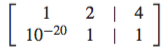
\includegraphics[width=3cm]{figs/2_3_Swamping-6} 
\end{figure}
将第一行乘以$-10^{-20}$加到第二行上得到
\begin{figure}
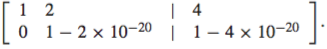
\includegraphics[width=5cm]{figs/2_3_Swamping-7} 
\end{figure}
\end{frame}


\begin{frame}
\frametitle{交换方程顺序后解方程组}
在IEEE双精度表示中$1- 2\times10^{-20}$与$1$相等,而$1- 4\times 10^{-20}$与$1$相等,所以方程变为
\begin{align}
x_1 + 2x_2 &= 4 \nonumber \\
            x_2 & =1,
\end{align}
进而得到$[x_1,x_2 ] = [2,1]$,与真实解非常接近。
\end{frame}


\begin{frame}
\frametitle{吞噬现象}
在第二种解法和第三种解法中,都存在大数吃掉小数的现象,但是第二种解法却产生了完全错误的解,而第三种解法却生成了近似度比较高的解,这是为什么呢?

这主要是因为第二种解法中,由于主元很小,我们需要将主元所在的方程乘以一个很大的数加到剩余方程中去,这种做法使得被消元的方程因为计算机的舍入误差而被主元所在的方程主导,也就是被吞噬了。换句话说,本来我们有两个方程存在,提供了两条独立的信息,由于这个主元消去使得第二个方程的信息几乎丢失了,因而得到了两个‘一样’的方程。

而对于第三种方法,虽然由于舍入误差主元所在方程的信息几乎没有带入到第二个方程中去,但是也因此保持了两个方程的独立性,所以得到了一个与真实解差距很小的解。

在高斯消元中,我们经常会遇到主元较小的情况,这里我们提供一种非常简便实用的方法,即部分主元消去,进而我们将会得到一种$LU$分解的改进形式。
\end{frame}


%%%%%%%%%%%%%%%%%%%%%%%%%%%%%%%%%%%%%%%%%%
\section{$PA = LU$分解}

\begin{frame}
\frametitle{部分主元消去}
为了避免吞噬现象,我们可以对基本的高斯消元法作一个简单的改进。例如在第一步的消元之前,我们首先比较第一列的所有元素,并选择满足
\begin{equation}
|a_{p1}| \ge |a_{i1}|, 1 \le i \le n,
\end{equation}
的第$p$行与第$1$行进行交换,之后再进行消去运算。通过这样的改进我们容易发现,消去第一列除第一行外的非零分元素过程中每一次的乘子
\begin{equation}
m_{i1} = \frac{a_{i1}}{a_{11}},
\end{equation}
都满足$|m_{i1}| \le 1$。

这样的主元的选取在消去过程中的每一步都进行一次,这样在消去中的每一个乘子$m_{ij}$的绝对值都会小于$1$,从而避免了吞噬现象的出现。
\end{frame}


\begin{frame}
\frametitle{部分主元消去}
我们用以下的例子来展示部分主元消去。
\begin{example}
解方程组
\begin{align}
x_1 - x_2 + 3 x_3 &= -3 \nonumber \\
- x_1 - 2 x_3 &= 1 \nonumber \\
2x_1 + 2x_2 + 4 x_3 &= 0
\end{align}
\end{example}
首先将方程写为增广矩阵形式
\begin{figure}
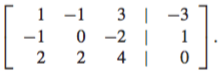
\includegraphics[width=4cm]{figs/2_4_P_Pivoting-1} 
\end{figure}
\end{frame}


\begin{frame}
\frametitle{部分主元消去}
选取第一列上绝对值最大的元$2$作为主元并交换第三行和第一行的顺序,得到
\begin{figure}
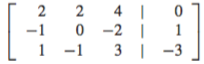
\includegraphics[width=4cm]{figs/2_4_P_Pivoting-2} 
\end{figure}
将第一行乘以$\frac{1}{2}$加到第二行得到
\begin{figure}
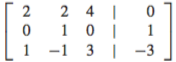
\includegraphics[width=4cm]{figs/2_4_P_Pivoting-3} 
\end{figure}
将第一行乘以$-\frac{1}{2}$加到第三行得到
\begin{figure}
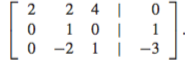
\includegraphics[width=4cm]{figs/2_4_P_Pivoting-4} 
\end{figure}
\end{frame}


\begin{frame}
\frametitle{部分主元消去}
在消去第二列时再次选取主元,将第二行与第三行交换,得到
\begin{figure}
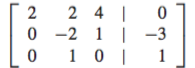
\includegraphics[width=3cm]{figs/2_4_P_Pivoting-5} 
\end{figure}
将第二行乘以$\frac{1}{2}$加到第三行得到
\begin{figure}
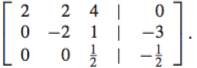
\includegraphics[width=3cm]{figs/2_4_P_Pivoting-6} 
\end{figure}
解方程
\begin{align}
2x_1 + 2 x_2 + 4 x_3 &= 0, \nonumber \\
-2x_2 + x_3 &= -3, \nonumber \\
\frac{1}{2}x_3 &= -\frac{1}{2}
\end{align}
得到$x = [1,1,-1]$。
\end{frame}


\begin{frame}
\frametitle{部分主元消去}
\begin{remark}
部分主元消去在遇到主元为$0$的时候也是适用的,但是如果在消去到第$i$步时,该列上$a_{ii}$以下的元素都为$0$,则消去失败。但这种情况对应的是系数矩阵为奇异矩阵,即系数矩阵不满秩的情况,这种情况下高斯消元不论作任何改进都是无法得到解的,因为此时方程存在无穷多组解。
\end{remark}
\end{frame}


\begin{frame}
\frametitle{重排矩阵}
对于部分选取主元的高斯消元法,我们也可以在某种意义下对系数矩阵作$LU$分解。这里我们首先要介绍重排矩阵。
\begin{definition}
如果一个$n \times n$的矩阵在每一行和每一列上除了一个元素为$1$外其它元素都为$0$,那么这个矩阵叫作重排矩阵(permutation matrix)。
\end{definition}
对于$n=2$,我们有两种重排矩阵
\begin{figure}
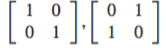
\includegraphics[width=3cm]{figs/2_4_Permutation_M-1} 
\end{figure}
对于$n = 3$,我们有六种重排矩阵
\begin{figure}
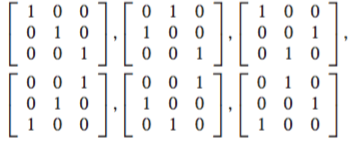
\includegraphics[width=4.5cm]{figs/2_4_Permutation_M-2} 
\end{figure}
\end{frame}


\begin{frame}
\frametitle{重排矩阵}
\begin{theorem}
如果将重排矩阵$P$看作是单位矩阵通过行交换得来的矩阵,则$PA$得到的矩阵相当于对矩阵$A$作同样的行交换所得到的矩阵。
\end{theorem}
例如重排矩阵
\begin{figure}
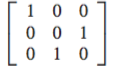
\includegraphics[width=2cm]{figs/2_4_Permutation_M-3} 
\end{figure}
可以看作将单位矩阵的第$2$行和第$3$行交换位置得来的,进而我们有
\begin{figure}
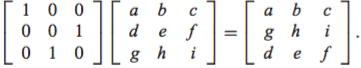
\includegraphics[width=6cm]{figs/2_4_Permutation_M-4} 
\end{figure}
\end{frame}


\begin{frame}
\frametitle{$PA = LU$分解}
$PA = LU$分解是$A$的行重排之后得到了$LU$分解,但是由于在消元过程开始的时候,我们并不知道$A$会经历怎样的重排过程,所以我们将相关信息储存下来,并随着行交换进行重排。这个过程可以由下面的例子很好的展示出来。

对$A$进行$PA = LU$分解,其中
\begin{figure}
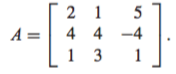
\includegraphics[width=3cm]{figs/2_4_PA-1} 
\end{figure}
\end{frame}


\begin{frame}
\frametitle{$PA = LU$分解}
首先对第一行的第二行进行交换得到
\begin{figure}
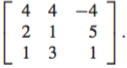
\includegraphics[width=3cm]{figs/2_4_PA-2} 
\end{figure}
此时重排矩阵$P$为
\begin{figure}
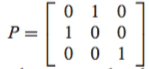
\includegraphics[width=3cm]{figs/2_4_PA-3} 
\end{figure}
\end{frame}


\begin{frame}
\frametitle{$PA = LU$分解}
将第$1$行乘以$-\frac{1}{2}$加到第$2$行,得到
\begin{figure}
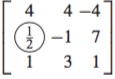
\includegraphics[width=2cm]{figs/2_4_PA-4} 
\end{figure}
将第$1$行乘以$-\frac{1}{4}$加到第$3$行,得到
\begin{figure}
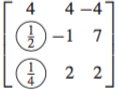
\includegraphics[width=2cm]{figs/2_4_PA-5} 
\end{figure}
注意到圆圈里面的数字,事实上这里展示的是实际运算之中所发生的事情,也就是说,在实际运算中我们在消元的同时也将消元产生的乘子储存在$A$对应的位置当中,这是因为这些位置上的元素因为已经被消去为$0$所以不会再被用到。
\end{frame}


\begin{frame}
\frametitle{$PA = LU$分解}
继续对第$2$列进行消元。首先将第$2$行与第$3$行交换位置,得到
\begin{figure}
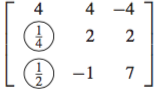
\includegraphics[width=3cm]{figs/2_4_PA-6} 
\end{figure}
此时重排矩阵$P$为
\begin{figure}
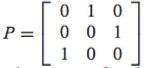
\includegraphics[width=3cm]{figs/2_4_PA-7} 
\end{figure}
我们注意到,圆圈里面的数字也随着行交换而交换,这就是我们之前提到的相关信息随着行交换进行重排。
\end{frame}


\begin{frame}
\frametitle{$PA = LU$分解}
将第$2$行乘以$\frac{1}{2}$加到第$3$行上,得到
\begin{figure}
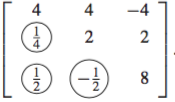
\includegraphics[width=3cm]{figs/2_4_PA-8} 
\end{figure}
这样我们就得到了$PA = LU$分解
\begin{figure}
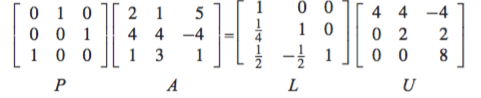
\includegraphics[width=8cm]{figs/2_4_PA-9} 
\end{figure}
\end{frame}


\begin{frame}
\frametitle{利用$PA = LU$分解解方程组}
当我们得到了方程组系数矩阵$A$的$PA = LU$分解后,我们也可以用它来解线性方程组,我们有
\begin{align}
PA x = Pb \nonumber \\
LU x = Pb.
\end{align}
因此我们将解方程组分为两步
\begin{align}
L y = Pb \nonumber \\
U x = y.
\end{align}
\end{frame}


\begin{frame}
\frametitle{$PA = LU$分解的Maltab实现}
Matlab具有强大的矩阵计算功能,尤其是在$PA = LU$分解这个问题上,我们只需要输入简单的$\rm{lu}$命令就可以得到一个矩阵的$PA = LU$分解,例如
\begin{figure}
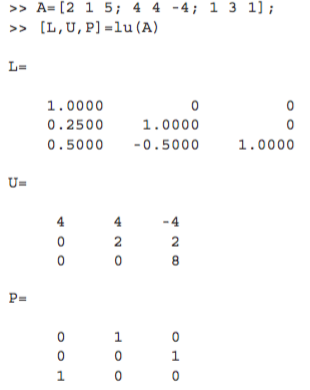
\includegraphics[width=4cm]{figs/2_4_PA-10} 
\end{figure}
\end{frame}

\begin{frame}
\frametitle{课后阅读}
[NA] 第2章 2.1,2.2,2.3.2,2.4


\end{frame}

\end{document}

